\chapter{Datasets and losses}
\label{chap:supervised_learning}

\begin{supportbox}{About this chapter}
This chapter formalizes the supervised learning scenario. We introduce the concepts of datasets, loss functions, and empirical risk minimization, stressing the basic assumptions made in supervised learning. We close by providing a probabilistic formulation of supervised learning built on the notion of maximum likelihood. This short chapter serves as the backbone for the rest of the book.
\end{supportbox}

\section{What is a dataset?}
\label{sec:dataset}

We consider a scenario in which manually coding a certain function is unfeasible (e.g., recognizing objects from real-world images), but gathering \textbf{examples} of the desired behaviour is sufficiently easy. Examples of this abound, ranging from speech recognition to robot navigation. We formalise this idea with the following definition.

\begin{definition}[Dataset] \addbottle
A \textbf{supervised dataset} $\mathcal{S}_n$ of size $n$ is a set of $n$ pairs $\mathcal{S}_n = \left\{(x_i, y_i)\right\}_{i=1}^n$, where each $(x_i, y_i)$ is an example of an input-output relationship we want to model. We further assume that each example is an \textbf{identically} and \textbf{independently} distributed (i.i.d.) draw from some unknown (and unknowable) probability distribution $p(x,y)$.
\end{definition}

See Appendix \ref{chap:probability_theory} if upon reading the definition you want to brush up on probability theory. The last assumption appears technical, but it is there to ensure that the relationship we are trying to model is meaningful. In particular, samples being \textbf{identically distributed} means that we are trying to approximate something which is sufficiently stable and unchanging through time. As a representative example, consider the task of gathering a dataset to recognise car models from photos. This assumption will be satisfied if we collect images over a short time span, but it will be invalid if collecting images from the last few decades, since car models will have changed over time. In the latter case, training and deploying a model on this dataset will fail as it will be unable to recognise new models or will have sub-optimal performance when used.

Similarly, samples being \textbf{independently distributed} means that our dataset has no bias in its collection, and it is sufficiently representative of the entire distribution. Going back to the previous example, gathering images close to a Tesla dealership will be invalid, since we will collect an overabundance of images of a certain type while loosing on images of other makers and models. Note that the validity of these assumptions depends on the context: a car dataset collected in Italy may be valid when deploying our model in Rome or Milan, while it may invalid when deploying our model in Tokyo or in Taiwan. The i.i.d. assumption should always be checked carefully to ensure we are applying our supervised learning tools to a valid scenario. Interestingly, modern LLMs are trained on such large distributions of data that even understanding what tasks are truly \textit{in-distribution} against what is \textit{out-of-distribution} (and how much the models are able to generalize) becomes blurred \cite{yuan2024revisiting}.

\subsection{Variants of supervised learning}
\label{subsec:variants_supervised_learning}

\begin{figure}[t]
    \centering
    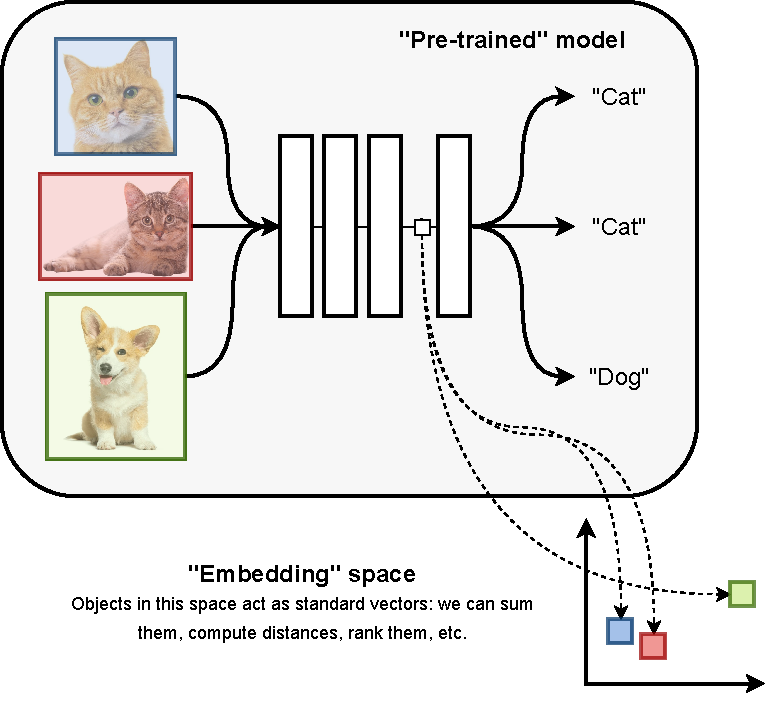
\includegraphics[width=0.7\textwidth]{images/embedding.pdf}
    \caption{Differentiable models process data by transforming it sequentially via linear algebra operations. In many cases, after we optimize these programs, the internal representations of the input data of the model (what we call a \textbf{pre-trained} model) have geometric properties: for example, semantically similar images are projected to points that are close in this “latent” space. Transforming data from a non-metric space (original input images) to a metric space (bottom right) is called \textbf{embedding} the data.}
    \label{fig:embedding}
\end{figure}

There exists many variations on the standard supervised learning scenario, although most successful applications make use of supervised learning in some form or another. For example, some datasets may not have available \textbf{targets} $y_i$, in which case we  talk about \textbf{unsupervised} learning. Typical applications of unsupervised learning are \textbf{clustering} algorithms, in which we want to aggregate our input data into \textit{clusters} such that points in a cluster are similar and points between clusters are dissimilar \cite{hastie2009elements}. As another example, in a \textbf{retrieval} system we may want to search a large database for the top-$k$ most similar elements to a user-given query.

When dealing with complex data such as images, this is non-trivial because distances on images are ill-defined if we operate on pixels (i.e., even small perturbations can modify millions of pixels). However, assume we have available some (differentiable) model that we have already optimized for some other task which we assume sufficiently generic, e.g., image classification. We call it a  \textbf{pre-trained} model. As we will see, the internal states of this model can be interpreted as vectors in a high-dimensional space. In many cases, these vectors are shown to have useful geometrical properties, in the sense that objects that are semantically similar are sent (\textbf{embedded}) into points that are close in these representations. Hence, we can use these latent representations with standard clustering models, such as Gaussian mixture models \cite{huang2014deep}. See Figure \ref{fig:embedding} for a high-level overview of this idea.

What if we do not have access to a pre-trained model? A common variation of unsupervised learning is called \textbf{self-supervised} learning (SSL, \cite{zbontar2021barlow}). The aim of SSL is to automatically find some supervised objective from a generic unsupervised dataset, in order to optimize a model that can be used in a large set of downstream tasks. For example, if we have access to a large corpus of text, we can always optimize a program to predict how a small piece of text is likely to continue \cite{radford2019language}. The realization that neural networks can also perform an efficient embedding of text  when pre-trained in a self-supervised way had a profound impact on the community \cite{mikolov2013distributed}.\footnote{Large-scale web datasets are also full of biases, profanity, and vulgar content. Recognizing that models trained on this data internalize these biases was another important realization \cite{bolukbasi2016man} and it is one of the major criticisms of closed-source foundation models \cite{bender2021dangers}.}

\begin{figure}[t]
    \centering
    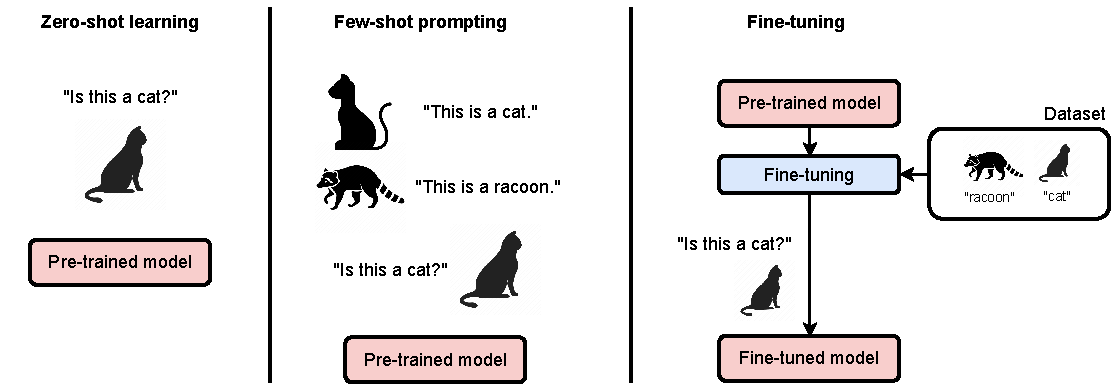
\includegraphics[width=0.95\textwidth]{images/using_models.pdf}
    \caption{Three ways of using trained models. \textbf{Zero-shot}: a question is directly given to the model. This can be achieved with generative language models (introduced in Chapter \ref{chap:convolutions_beyond_images}). \textbf{Few-shot prompting} is similar, but a few examples are provided as input. Both techniques can be employed only if the underlying model shows a large amount of generalization capabilities. \textbf{Fine-tuning}: the model is optimized via gradient descent on a small dataset of examples. This proceeds similarly to training the model from scratch.}
    \label{fig:using_models}
\end{figure}

As we will see in Chapter \ref{chap:convolutions_beyond_images} and Chapter \ref{chap:transformers}, LLMs can be seen as modern iterations on this basic idea, since optimizing models such as GPT or Llama \cite{touvron2023llama} always start by a basic self-supervised training in terms of next-token prediction. These models are sometimes called \textbf{foundation models}. In the simplest case, they can be used out-of-the-box for a new task, such as answering a query: in this case, we say they are used in a \textbf{zero-shot} fashion. For LLMs, it is also possible to provide a small number of examples of a new task as input prompt, in which case we talk about \textbf{few-shot prompting}. In the most general case, we can take a pre-trained foundation model and optimize its parameters by gradient descent on a new task: this is called \textbf{fine-tuning} the model. See Figure \ref{fig:using_models} for a comparison of the three approaches. In this book we focus on building models from scratch, but fine-tuning can be done by similar means.

Fine-tuning is made especially easy by the presence of large open-source repositories online.\footnote{\url{https://huggingface.co/models}} Fine-tuning can be done on the full set of parameters of the starting model, or by considering only a smaller subset or a small number of additional parameters: this is called \textbf{parameter-efficient fine-tuning} (PEFT) \cite{lialin2023scaling}.\footnote{Few-shot learning can also be done by fine-tuning the model. In cases in which fine-tuning is not needed, we say the model is performing \textbf{in-context learning} \cite{akyurek2022learning}.} We will consider PEFT techniques in the next volume.

Many other variations of supervised learning are possible, which we do not have space to list in detail here except for some generic hints. If only parts of a dataset are labeled, we have a \textbf{semi-supervised} scenario \cite{belkin2006manifold}. We will see some examples of semi-supervised learning in Chapter \ref{chap:gnns}. Additionally, we can have scenarios with multiple datasets belonging to “similar” distributions, or the same distribution over different period of times, giving rise to countless tasks depending on the order in which the tasks or the data are provided, including \textbf{domain adaptation}, \textbf{meta-learning} \cite{finn2017model}, \textbf{continual learning} \cite{parisi2019continual,biesialska2020continual}, \textbf{metric learning}, \textbf{unlearning}, etc. Some of these will be treated in the next volume.

\begin{supportbox}{More on the i.i.d. property}
Importantly, ensuring the i.i.d. property is not a one-shot process, and it must be checked constantly during the lifetime of a model. In the case of car classification, if unchecked, subtle changes in the distribution of cars over time will degrade the performance of a machine  learning model, an example of \textbf{domain shift}. As another example, a recommender system will change the way users interact with a certain app, as they will start reacting to suggestions of the recommender system itself. This creates \textbf{feedback loops} \cite{cinus2022effect} that require constant re-evaluation of the performance of the system and of the app.
\end{supportbox}

\section{Loss functions}
\label{sec:loss_functions}

\addclock Once data has been gathered, we need to formalize our idea of “approximating” the desired behavior, which we do by introducing the concept of \textbf{loss functions}.

\begin{definition}[Loss function] \addbottle
Given a desired target $y$ and the predicted value $\hat{y}=f(x)$ from a model $f$, a \textbf{loss function} $l(y, \hat{y}) \in \mathbb{R}$ is a scalar, differentiable function whose value correlates with the performance of the model, i.e., $l(y, \hat{y}_1) < l(y, \hat{y}_2)$ means that the prediction $\hat{y}_1$ is better than the prediction $\hat{y}_2$ when considering the reference value (target) $y$.
\end{definition}

A loss function embeds our understanding of the task and our preferences in the solutions’ space on a real-valued scale that can be exploited in an optimization algorithm. Being differentiable, it allows us to turn our learning problem into a mathematical optimization problem that can be solved via gradient descent by minimizing the average loss on our dataset.

To this end, given a dataset $\mathcal{S}_n = \left\{(x_i, y_i)\right\}$ and a loss function $l(\cdot, \cdot)$, a sensible optimization task to solve is the minimum average loss on the dataset achievable by any possible \textit{differentiable} model $f$:

\vspace{1em}
\begin{equation}
    f^* = \underset{f}{\arg\min} \;\; \eqnmarkbox[drawred]{node}{\frac{1}{n}\sum_{i=1}^n} l(y_i, \eqnmarkbox[drawblue]{node2}{f(x_i)})
    \label{eq:empirical_risk_minimization}
\end{equation}
\annotate[yshift=1em]{above,right}{node}{Average over the dataset}
\annotate[yshift=-1.5em]{below,left}{node2}{Prediction of $f$ on the $i$-th  sample from the dataset}

\vspace{1em}
For historical reasons, \eqref{eq:empirical_risk_minimization} is referred to as \textbf{empirical risk minimization} (ERM), where \textit{risk} is used as a generic synonym for \textit{loss}. See also the box in the next page for more on the origin of the term.

In \eqref{eq:empirical_risk_minimization} we are implicitly assuming that we are minimizing across the space of all possible functions defined on our input $x$. We will see shortly that our models can always be parameterized by a set of tensors $w$ (called \textbf{parameters} of the model), and minimization is done by searching for the optimal value of these parameters via numerical optimization, which we denote by $f(x,w)$. Hence, given a dataset $\mathcal{S}_n$, a loss function $l$, and a model space $f$, we can \textbf{train} our model by optimizing the empirical risk \eqref{eq:empirical_risk_minimization} via gradient descent \eqref{eq:gradient_descent}:
%
\begin{equation}
    {\color{drawred}w^*} = \underset{w}{\arg\min} \;\; \frac{1}{n}\sum_{i=1}^n l(y_i, f(x_i, {\color{drawred}w}))
    \label{eq:empirical_risk_minimization_2}
\end{equation}
%
where the minimization is now done with respect to the parameter's tensor $w$.

\subsection*{On the differentiability of the loss}
\label{subsec:differentiability_loss}

 Before proceeding, we make two observations on the ERM framework. \addteacup First, note that the differentiability requirement on $l$ is fundamental. Consider a simple \textbf{binary classification} task (that we will introduce properly in the next chapter), where $y \in \left\{-1,+1\right\}$ can only take two values, $-1$ or $1$. Given a real-valued model $f(x) \in \mathbb{R}$, we can equate the two decisions with the sign of $f$ -- which we denote as $\text{sign}(f(x))$ -- and define a \textbf{0/1 loss} as:
%
\begin{equation}
l(y, \hat{y})=\begin{cases} 0 & \text{ if } \text{sign}(\hat{y}) = y \\ 1 & \text{ otherwise } \end{cases}
\label{eq:01_loss}
\end{equation}
%
While this aligns with our intuitive notion of “being right”, it is useless as loss function since its gradient will almost always be zero (except when the sign of $f$ switches), and any gradient descent algorithm will remain stuck at initialization. A less intuitive quantity in this case is the \textbf{margin} $y\hat{y}$, which is positive [negative] depending on whether the sign of the model aligns [or does not align] with the desired one, but it varies continuously differently from 0/1 loss in \eqref{eq:01_loss}. 

A possible loss function in this case is the \textbf{hinge loss} $l(y,\hat{y}) = \max(0, 1 - y\hat{y})$, which is used to train support-vector models. Details apart, this shows the inherent tension between designing loss functions that encode our notion of performance while at the same time being useful for numerical optimization.

\subsection{Expected risk and overfitting}

As a second observation, note that the empirical risk is always trivial to minimize, by defining:

\begin{equation}
f(x) = \begin{cases} y & \text{ if } \eqnmarkbox[drawred]{node}{(x,y) \in \mathcal{S}_n} \\ \eqnmarkbox[drawblue]{node2}{\bar{y}} & \text{ otherwise} \end{cases} \;.
\label{eq:lookup_table}
\end{equation}
\annotate[yshift=1em]{above,right}{node}{$x$ is in the training set}
\annotate[yshift=-1em]{below,right}{node2}{Default value, e.g., $0$}

\vspace{1em}
This is a look-up table that returns a prediction $y$ if the pair $(x,y)$ is contained in the dataset, while it defaults to some constant prediction $\bar{y}$ (e.g., 0) otherwise. Assuming that the loss is lower-bounded whenever $y = \hat{y}$, this model will always achieve the lowest possible value of empirical risk, while providing no actual practical value. 

This shows the difference between \textbf{memorization} and \textbf{learning} (optimization). Although we search for a model by optimizing some average loss quantity on our training data, as in \eqref{eq:empirical_risk_minimization}, our true objective is minimizing this quantity on some unknown, future input yet to be seen. The elements of our training set are only a proxy to this end. We can formalize this idea by defining the \textbf{expected risk minimization} problem.

\begin{definition}[Expected risk]
Given a probability distribution $p(x,y)$ and a loss function $l$, the \textbf{expected risk} (ER) is defined as:
%
\begin{equation}
\textnormal{ER}[f] = \mathbb{E}_{p(x,y)}\left[ l(y, f(x)) \right]
\label{eq:expected_risk}
\end{equation}
\end{definition}

Minimizing \eqref{eq:expected_risk} can be interpreted as minimizing the average (expected) loss across \textit{all possible input-output pairs} (e.g., all possible emails) that our model could see. Clearly, a model with low expected risk would be guaranteed to work correctly. However, the quantity in \eqref{eq:expected_risk} is unfeasible to compute in practice, as enumerating and labeling all data points is impossible. The empirical risk provides an estimate of the expected risk under the choice of a given dataset and can be seen as a Monte Carlo approximation of the ER term.

The difference in loss between the expected and the empirical risk is called the \textbf{generalization gap}: a pure memorization algorithm like \eqref{eq:lookup_table} will have poor generalization or, in other terms, it will \textbf{overfit} to the specific training data we provided. Generalization can be tested in practice by keeping a separate \textbf{test dataset} $\mathcal{T}_m$ with $m$ data points never used during training, $\mathcal{S}_n \cap \mathcal{T}_m = \emptyset$. Then, the difference in empirical loss between $\mathcal{S}_n$ and $\mathcal{T}_m$ can be used as an approximate measure of overfitting.

\begin{supportbox}{Risk and loss}
Empirical and expected risk minimization framed in this way are generally associated with the work of the Russian computer scientist V. Vapnik \cite{vapnik2013nature}, which gave rise to the field of \textit{statistical learning theory} (SLT). SLT is especially concerned with the behaviour of \eqref{eq:empirical_risk_minimization} when seen as a finite-sample approximation of \eqref{eq:expected_risk} under some restricted class of functions $f$ and measure of underlying complexity \cite{poggio2003mathematics,shalev2014understanding,mohri2018foundations}. The counter-intuitive properties of modern neural networks (such as strong generalization long after overfitting should have been expected) have opened many new avenues of research in SLT \cite{poggio2020theoretical}. See also the introduction of Chapter \ref{chap:deep_cnns}.
\end{supportbox}

\subsection{How to select a valid loss function?} 
\label{subsec:how_to_select_a_loss}

\begin{tcolorbox}
If you have not done so already, this is a good time to study (or skim) the material in Appendix \ref{chap:probability_theory}, especially probability distributions, sufficient statistics, and maximum likelihood estimation.
\end{tcolorbox}

As we will see in the next chapters, the loss encodes our a priori knowledge on the task to be solved, and it has a large impact on performance. In some cases, simple considerations on the problem are enough to design valid losses (e.g., as done for the hinge loss in Section \ref{subsec:differentiability_loss}).

However, it is possible to work in a more principled fashion by reformulating the entire training process in purely probabilistic terms, as we show now. This formulation provides an alternative viewpoint on learning, which may be more intuitive or more useful in certain scenarios. It is also the preferred viewpoint of many books \cite{bishop2024deep}. We provide the basic ideas in this section, and we consider specific applications later on in the book.

The key observation is the following. In Section \ref{sec:dataset}, we started by assuming that our examples come from a distribution $p(x, y)$. By the product rule of probability, we can decompose $p(x,y)$ as $p(x,y) = p(x)p(y \mid x)$, such that $p(x)$ depends on the probability of observing each input $x$, and the conditional term $p(y \mid x)$ describes the probability of observing a certain output $y$ given an input $x$.\footnote{We can also decompose it as $p(x, y) = p(x \mid y)p(y)$. Methods that require to estimate $p(x)$ or $p(x \mid y)$ are called \textbf{generative}, while methods that estimate $p(y \mid x)$ are called \textbf{discriminative}. Apart from language modeling, in this book we focus on the latter case. We consider generative modelling more broadly in the next volume.} Approximating $p(y \;\vert\; x)$ with a function $f(x)$ makes sense if we assume that the probability mass is mostly concentrated around a single point $y$, i.e., $p(y \;\vert\; x)$ is close to a so-called Dirac delta function, and it drastically simplifies the overall problem formulation.

However, we can relax this by assuming that our model $f(x)$ does not provide directly the prediction, but it is used instead to parameterize the sufficient statistics of a conditional probability distribution $p(y \mid f(x))$ over possible outputs. For example, consider a classification problem where $y \in \left\{1,2,3\right\}$ can take three possible values. We can assume our model has three outputs that parameterize a categorical distribution over these classes, such that:
%
$$
p(\mathbf{y} \;\vert\; f(x)) = \prod_{i=1}^3 {f_i(x)}^{y_i}
$$
%
where $\mathbf{y} \sim \text{Binary}(3)$ is the one-hot encoding of the class $y$\footnote{Given an integer $i$, its one-hot representation is a vector of all zeros except the $i$-th element, which is $1$. This is introduced formally in Section \ref{sec:linear_models_for_classification}.} and $f(x) \sim \Delta(3)$ are the predicted probabilities for each class. As another example, assume we want to predict a single scalar value $y \in \mathbb{R}$ (\textbf{regression}). We can model this with a two-valued function $f(x) \sim (2)$ such that the prediction is a Gaussian with appropriate mean and variance:

\begin{equation}
p(y \;\vert\; f(x))=\mathcal{N}(y \mid f_1(x), \eqnmarkbox[drawred]{node}{f_2^2(x)})
\label{eq:gaussian_conditional_distribution}
\end{equation}
\annotate[yshift=-1em]{below,right}{node}{Squared to ensure positivity}

\vspace{1em}
where the second output of $f(x)$ is squared to ensure that the predicted variance remains positive. As can be seen, this is a very general setup that subsumes our previous discussion, and it provides more flexibility to the designer, as choosing a specific parameterization for $p(y \;\vert\; x)$ can be easier than choosing a specific loss function $l(y, \hat{y})$. In addition, this framework provides a more immediate way to model uncertainty, such as the variance in \eqref{eq:gaussian_conditional_distribution}.
%
\subsection{Maximum likelihood}
%
How can we train a probabilistic model? Remember that we assumed the samples in our dataset $\mathcal{S}_n$ to be i.i.d. samples from a probability distribution $p(x,y)$. Hence, given a model $f(x)$, the probability assigned to the dataset itself by a specific choice $f$ of function is given by the product of each sample in the dataset:
%
$$
p(\mathcal{S}_n \;\vert\; f)=\prod_{i=1}^n p(y_i \;\vert\; f(x_i))
$$

The quantity $p(\mathcal{S}_n  \;\vert\; f)$ is called the \textbf{likelihood} of the dataset. For a random choice of $f(x)$, the model will assign probabilities more or less at random across all possible inputs and outputs, and the likelihood of our specific dataset will be small. A sensible strategy, then, is to select the model such that the likelihood of the dataset is instead maximized. This is a direct application of the maximum likelihood approach (see Section \ref{sec:maximum_likelihood_estimation} in Appendix \ref{chap:probability_theory}).

\begin{definition}[Supervised learning as maximum likelihood] \addbottle
Given a dataset $\mathcal{S}_n = \left\{(x_i, y_i)\right\}$ and a family of probability distributions $p(y \;\vert\; f(x))$ parameterized by $f(x)$, the \textbf{maximum likelihood} (ML) solution is given by:
%
$$
f^* = \underset{f}{\arg\max}\prod_{i=1}^n p(y_i \;\vert\; f(x_i)) \,.
$$
\end{definition}

While we are again left with an optimization problem, it now follows directly from the laws of probability once all probability distributions are chosen, which is in contrast to before, where the specific loss was part of the design space. The two viewpoints, however, are closely connected. Working in log-space and switching to a minimization problem we obtain:
%
$$
\underset{f}{\arg\max} \left\{ \log \prod_{i=1}^n p(y_i \;\vert\; f(x_i)) \right\} = \underset{f}{\arg\min} \left\{ \sum_{i=1}^n -\log(p(y_i \;\vert\; f(x_i)) \right\}
$$
%
Hence, the two formulations are identical if we identify $-\log(p(y \;\vert\; f(x))$ as a “pseudo-loss” to be optimized. As we will see, all loss functions used in practice can be obtained under the ML principle for specific choices of this term. Both viewpoints are interesting, and we urge readers to keep them in mind as we progress in the book.

\section{Even more probability: Bayesian learning}
\label{sec:bayesian_learning}

\addteacup We discuss here a further generalization of the probabilistic formulation called \textbf{Bayesian neural networks} (BNNs), which is of interest in the literature. We only provide the general idea and we refer the reader to one of many in-depth tutorials, e.g., \cite{jospin2022hands}, for more details.

By designing a probability function $p(y \;\vert\; f(x))$ instead of $f(x)$ directly, we can handle situations where more than one prediction is of interest (i.e., the probability function has more than a single mode). However, our procedure still returns a \textit{single function} $f(x)$ out of the space of all possible functions, while it may happen than more than a single parameterization across the entire model’s space is valid. In this case, it could be useful to have access to all of them for a more faithful prediction.

Once again, we can achieve this objective by designing another probability distribution and then letting the rules of probability guide us. Since we are now planning to obtain a distribution across all possible functions, we start by defining a \textbf{prior probability distribution} $p(f)$ over all possible functions (once again, remember than in the rest of the book $f$ will be described by a finite set of parameters, in which case the prior $p(f)$ would be a prior over these weights). For example, we will see that in many situations functions with smaller norm are preferred (as they are more stable), in which case we could define a prior $p(f) \propto \frac{1}{\lVert f \rVert}$ for some norm $\lVert f \rVert$ of $f$. 

Once a dataset is observed, the probability over $f$ shifts depending on the prior and the likelihood, and the update is given by \textbf{Bayes’ theorem}:

\vspace*{1em}
\begin{equation}
\eqnmarkbox[drawblue]{node2}{p(f \;\vert\; \mathcal{S}_n)}=\frac{p(\mathcal{S}_n \;\vert\; f)\eqnmarkbox[drawred]{node}{p(f)}}{p(\mathcal{S}_n)}
\label{eq:posterior_distribution}
\end{equation}
\annotate[yshift=1em]{above,left}{node}{Prior (\textit{before} observing the dataset)}
\annotate[yshift=-1em]{below,right}{node2}{Posterior (\textit{after} observing the dataset)}

\vspace{1em}
The term $p(f \;\vert\; \mathcal{S}_n)$ is called the \textbf{posterior distribution function}, while the term $p(\mathcal{S}_n)$ in the denominator is called the \textbf{evidence} and it is needed to ensure that the posterior is properly normalized. Assume for now that we have access to the posterior. Differently from before, the distribution can encode preference for more than a single function $f$, which may provide better predictive power. Given an input $x$, we can make a prediction by averaging all possible models based on their posterior’s weight:

\vspace{1em}
\begin{equation}
p(y \;\vert\; x)=\int_f \eqnmarkbox[drawred]{node}{p(y \;\vert\; f(x))}\eqnmarkbox[drawblue]{node2}{p(f \;\vert\; \mathcal{S}_n)} \approx \eqnmarkbox[drawgreen]{node3}{\frac{1}{k}\sum_{i=1}^k} p(y \;\vert\; f_i(x))p(f_i \;\vert\; \mathcal{S}_n)
\label{predictive_distribution}
\end{equation}
\annotate[yshift=1em]{above,left}{node}{Prediction of $f(x)$}
\annotate[yshift=1.5em]{above,right}{node2}{Weight assigned to $f$}
\annotate[yshift=-1em]{below,right}{node3}{Monte Carlo approximation}

\vspace{1em}
where on the right term of \eqref{predictive_distribution} we have approximated the integral with a Monte Carlo average over $k$ random samples from the posterior distribution $f_k \sim p(f \;\vert\; \mathcal{S}_n)$. The overall beauty of this setup is marred by the fact that the posterior is in general impossible to compute in closed-form, except for very specific choices of prior and likelihood \cite{bishop2006pattern}. Lacking this, one is forced to approximated solutions, either by \textbf{Markov chain Monte Carlo} or by \textbf{variational inference} \cite{jospin2022hands}. We will see in Section \ref{subsec:dropout} one example of Bayesian treatment of the model's parameters called \textbf{Monte Carlo dropout}.

We remark on two interesting facts about the posterior before closing this section. First, suppose we are only interested about the function having highest posterior density. In this case, the evidence term can be ignored and the solution decomposed into two separate terms:

\begin{gather}
f^*=\underset{f}{\arg\max} \; p(\mathcal{S}_n \;\vert\; f)p(f) = \\ \underset{f}{\arg\max} \; \left\{\eqnmarkbox[drawred]{node}{\log p(\mathcal{S}_n \;\vert\; f)} + \eqnmarkbox[drawblue]{node2}{\log p(f)}\right\}
\end{gather}
\annotate[yshift=-1em]{below,left}{node}{Likelihood term}
\annotate[yshift=-1em]{below,right}{node2}{Regularization term}

This is called the \textbf{maximum a posteriori} (MAP) solution. If all functions have the same weight a priori (i.e., $p(f)$ is uniform over the function’s space), then the second term is a constant and the problem reduces to the maximum likelihood solution. In general, however, the MAP solution will impose a penalty to functions deviating too much from our prior distribution. We will see this is a useful idea to combat overfitting and impose specific constraints on the function $f$. The term $\log p(f)$ is generally called a \textbf{regularizer} over the function’s space as it pushes the solution towards the basin of attraction defined by the prior distribution.\footnote{The difference between maximum likelihood and maximum a posteriori solutions is loosely connected to the difference between the \textbf{frequentist} and \textbf{Bayesian} interpretation of probability \cite{hackenberger2019bayes}, i.e., probabilities as frequency of events or probabilities as a measure of uncertainty. From a very high-level point of view, ML sees the parameters as an unknown fixed term and the data as a random sample, while a Bayesian treatment sees the data as fixed and the parameters as random variables.} 

Second, the full Bayesian treatment provides a simple way to incorporate new data, e.g., a new dataset $\mathcal{S}^\prime_n$ from the same distribution. To do that, we replace the prior function in \eqref{eq:posterior_distribution} with the posterior distribution that we computed on the first portion of the dataset, which now represents the starting assumption on the possible values of $f$ which gets updated
by looking at new data.\footnote{Think of the original prior function as the distribution on $f$ after having observed an initial \textit{empty set} of values.} This can mitigate issues when training models online, most notably the so-called \textit{catastrophic forgetting} of old information \cite{kirkpatrick2017overcoming}.